\documentclass[a4paper, 10pt]{article}
\usepackage[utf8]{inputenc}
\usepackage[spanish]{babel}
\usepackage{graphicx}
\usepackage{geometry}
\usepackage{listings}
\usepackage{amsmath}
\usepackage{amsfonts}
\usepackage{amssymb}
\usepackage{caratula}
\usepackage[section]{placeins}
\usepackage{titlesec}

\setcounter{secnumdepth}{4}

\titleformat{\paragraph}
{\normalfont\normalsize\bfseries}{\theparagraph}{1em}{}
\titlespacing*{\paragraph}
{0pt}{3.25ex plus 1ex minus .2ex}{1.5ex plus .2ex}

\newcommand{\Z}{\mathbb{Z}}
\def\code#1{\texttt{#1}}
\newcommand\tab[1][0.5cm]{\hspace*{#1}}

\geometry{a4paper, margin=0.7in}

\begin{document}
    %Caratula
    \pagenumbering{gobble}
    \newpage

    \begin{center}
        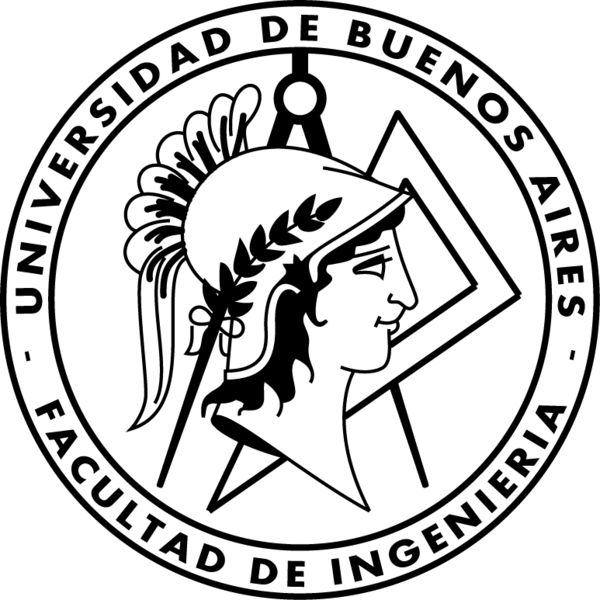
\includegraphics{images/logo}
    \end{center}

    \materia{Organización de Datos}
    \submateria{Segundo Cuatrimestre 2017}
    \titulo{Trabajo Práctico 1}
    \subtitulo{\textit{Análisis Exploratorio de Properati}}

    \integrante{Rodrigo De Rosa}{97799}{rodrigoderosa@outlook.com}
    \integrante{Marcos Schapira}{97934}{schapiramarcos@gmail.com}
    \integrante{Facundo Guerrero}{97981}{facundoiguerrero@gmail.com}
    \maketitle
    %Fin caratula
    %Table of contents
    \newpage
    \pagenumbering{roman}
    \tableofcontents
    %Fin table of contents
    %Informe
    \newpage
	\pagenumbering{arabic}
	\part{Análisis con Google Places}
		En este segmento se utilizo la API de Google Places 
		\footnote{https://developers.google.com/places/?hl=es-419} para obtener información adicional 
		sobre las propiedades provistas por Properati. Esta API permite entre otras cosas buscar 
		sitios (definidos en esta API como establecimientos, ubicaciones geográficas o puntos de 
		interés destacados) dentro de un área definida, como los límites de un mapa o alrededor de 
		un punto fijo. Para poder utilizarla sin embargo, se necesitan de coordenadas del tipo 
		latitud y longitud.\\ 
		El set de datos provistos contiene algunas ubicaciones en este formato pero no todas. 
		Por suerte dentro del set de datos está la información denominada como “geoname$\_$id”. 
		Este tipo de identificación pertenece a una base de datos geográfica con mas de 10 
		millones de entradas únicas. 
		Mediante la base de datos completa descargada de Kaggle
		\footnote{https://www.kaggle.com/geonames/geonames-database} se completaron las 
		latitudes y longitudes faltantes para así tener una muestra completa mayor.\\
		Para realizar pedidos a Google Places es necesario tener una API Key que esencialmente 
		controla el trafico diario de pedidos a la API. Esta limitación, utilizando una cuenta 
		prioritaria, es de 150000 pedidos por día. A la vez el tiempo entre que se realiza un 
		pedido y se obtiene su respuesta es muy alto. Es por esto que se limitaron las búsquedas 
		a las siguientes categorías(cantidades por propiedad en un radio de 400 metros):
		
		\begin{itemize}
		\item \emph{Locales de tipo gastronómico}
			\subitem Categorías de Google Places: \code{FOOD, BAKERY, BAR, MEAL$\_$TAKEAWAY, MEAL$\_$DELIVERY, RESTAURANT}
		\item \emph{Instituciones educativas}
			\subitem Categorías de Google Places: \code{SCHOOL, UNIVERSITY}
		\item \emph{Puntos de interés cultural} 
			\subitem Categorías de Google Places: \code{ART$\_$GALLERY, MUSEUM, PLACE$\_$OF$\_$WORSHIP}
		\item \emph{Espacios verdes} 
			\subitem Categorías de Google Places: \code{PARK, NATURAL$\_$FEATURE}
		\item \emph{Estaciones/Paradas de transporte publico}
			\subitem Categorías de Google Places: \code{BUS$\_$STATION, SUBWAY$\_$STATION}			
		\end{itemize}
		
		\section{Análisis Instituciones Educativas}
			\emph{A continuación se encuentra el análisis de las instituciones educativas para un set 
			de datos completo de 72474 entradas.}
			\subsection{Análisis del Precio por Metro Cuadrado}
				Para los siguientes gráficos se agruparon las propiedades por cantidad de instituciones 
				cercanas y sacando el promedio del precio por metro cuadrado para ellas. 
				Para que los resultados sean significativos, 
				se filtro a todas los conjuntos de propiedades con menos de 300 entradas para las 
				cantidades de instituciones cercanas. Por ejemplo: Si solo hay 15 propiedades con 
				60 instituciones cercanas, estas no se tuvieron en cuenta para el análisis.
				\begin{figure}
    				\centering
    				\makebox[\textwidth]{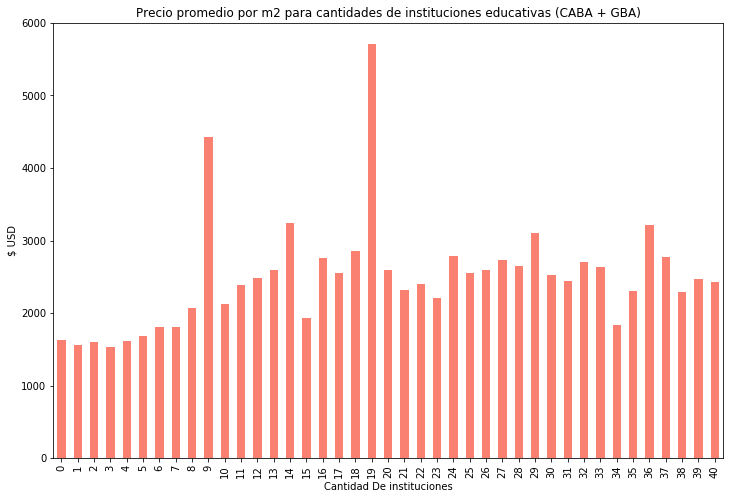
\includegraphics[width=\textwidth]{images/1}}
    				\caption{CABA + GBA}
				\end{figure}
				\begin{figure}
    				\centering
    				\makebox[\textwidth]{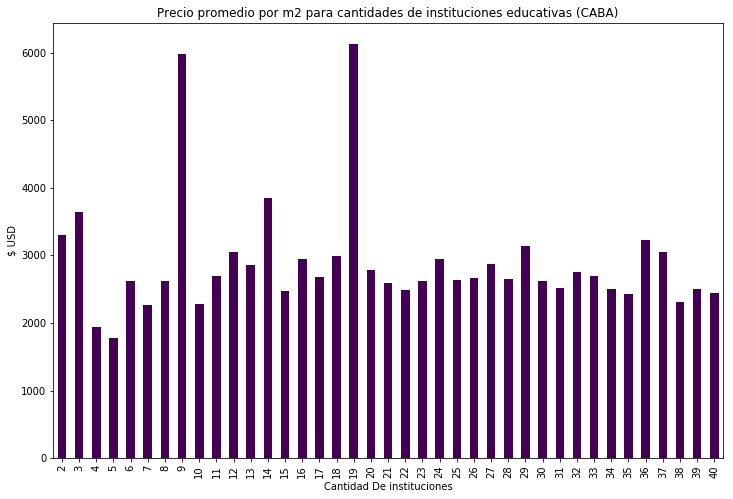
\includegraphics[width=\textwidth]{images/2}}
    				\caption{CABA}
				\end{figure}
				\begin{figure}
    				\centering
    				\makebox[\textwidth]{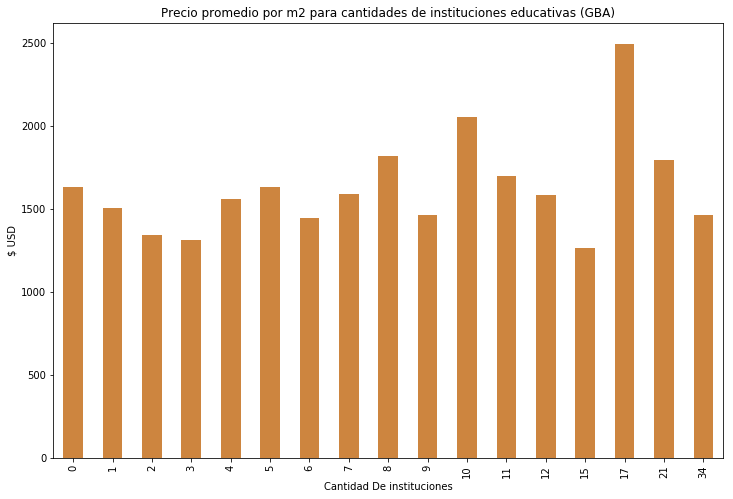
\includegraphics[width=\textwidth]{images/3}}
    				\caption{GBA}
				\end{figure}
				\FloatBarrier												
				
				Como se puede observar en los tres gráficos, hay una tendencia de un pico máximo 
				en todos para una cantidad de instituciones cercana a 20 instituciones. 
				Es importante notar sin embargo, que dichos máximos son muy distintos siendo el 
				de CABA casi el triple que el de GBA (6000 contra 2400 respectivamente).\\
				Se procede a aislarlas y observar en que zonas se concentran.\\
				
				\begin{figure}
    				\centering
    				\textbf{HEATMAP por ubicaciones}\par\medskip
    				\makebox[\textwidth]{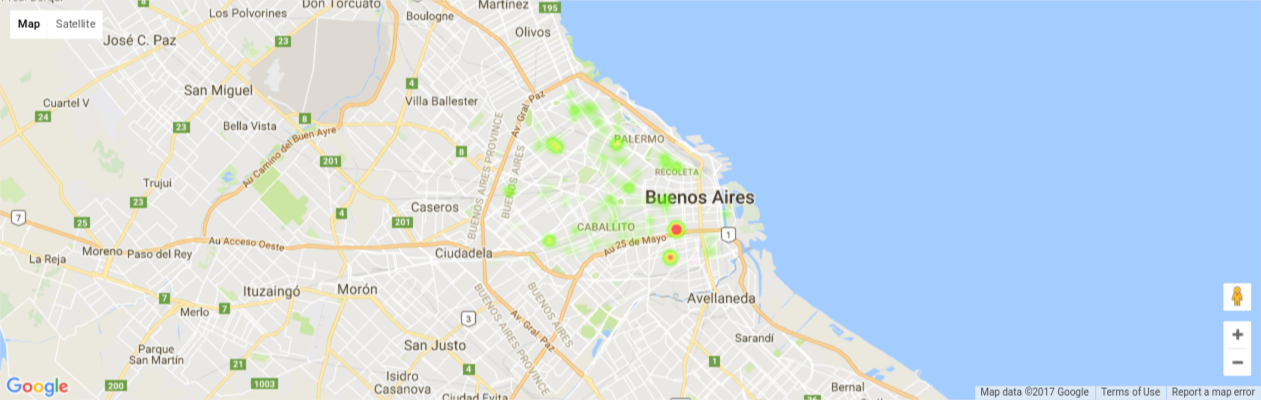
\includegraphics[width=\textwidth]{images/4}}
    				\caption{CABA con 19 instituciones}
				\end{figure}				
				\begin{figure}
    				\centering
    				\textbf{HEATMAP por precio del metro cuadrado}\par\medskip
    				\makebox[\textwidth]{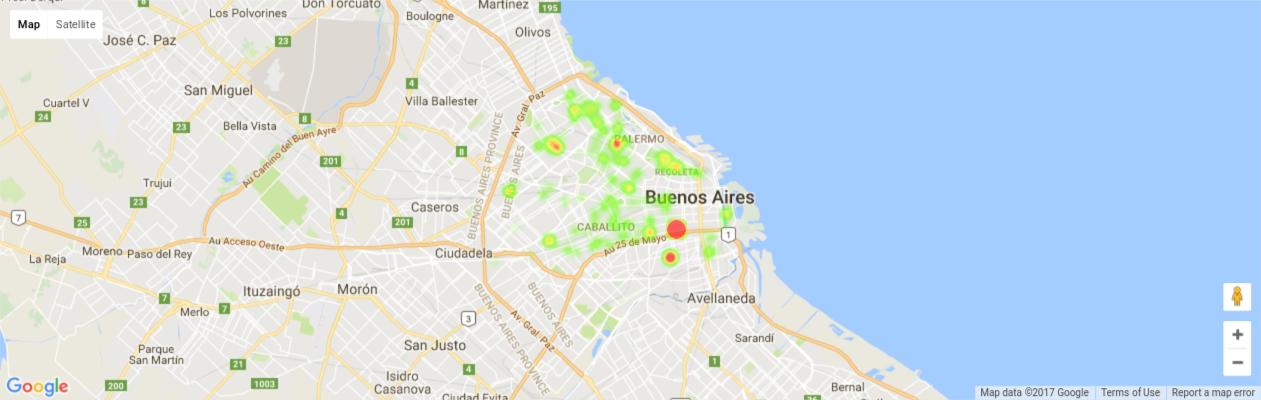
\includegraphics[width=\textwidth]{images/5}}
    				\caption{CABA con 19 instituciones}
				\end{figure}				
				\begin{figure}
    				\centering
    				\textbf{HEATMAP por ubicaciones}\par\medskip
    				\makebox[\textwidth]{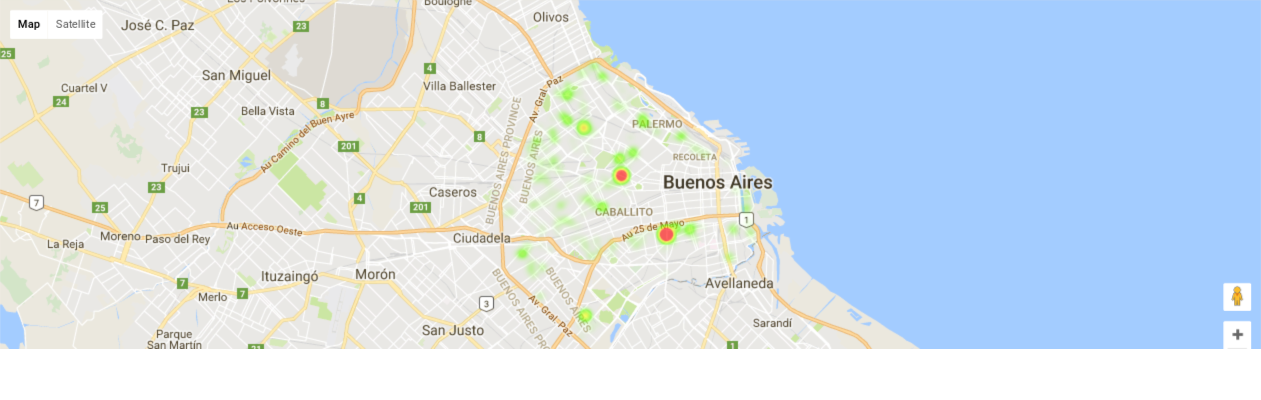
\includegraphics[width=\textwidth]{images/6}}
    				\caption{CABA con 9 instituciones}
				\end{figure}				
				\begin{figure}
    				\centering
    				\textbf{HEATMAP por precio del metro cuadrado}\par\medskip
    				\makebox[\textwidth]{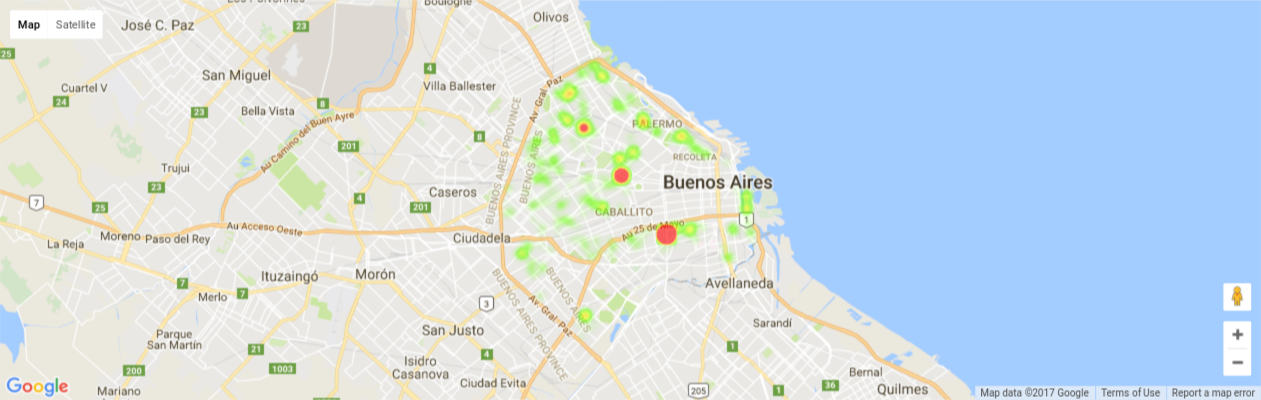
\includegraphics[width=\textwidth]{images/7}}
    				\caption{CABA con 9 instituciones}
				\end{figure}				
				\begin{figure}
    				\centering
    				\textbf{HEATMAP por ubicaciones}\par\medskip
    				\makebox[\textwidth]{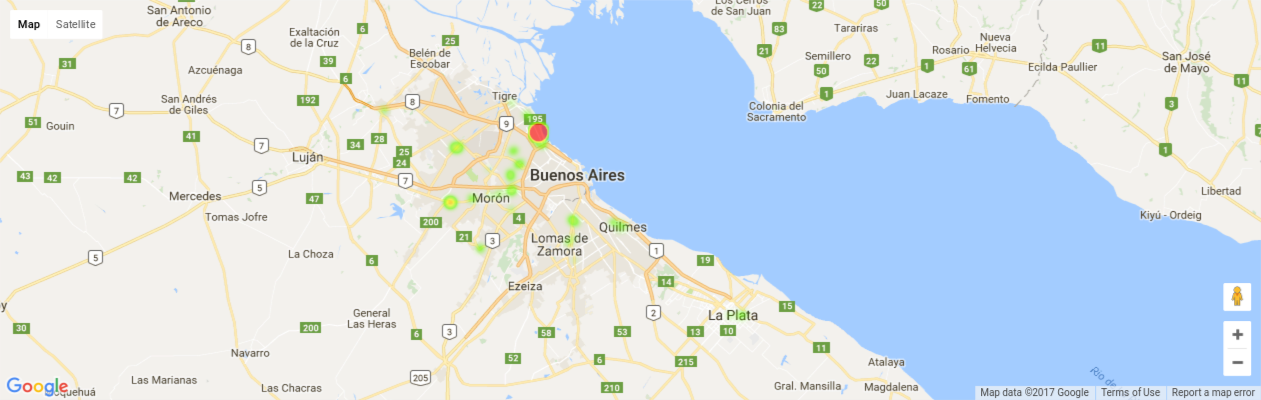
\includegraphics[width=\textwidth]{images/8}}
    				\caption{GBA con 17 instituciones}
				\end{figure}
				\begin{figure}
    				\centering
    				\textbf{HEATMAP por precio del metro cuadrado}\par\medskip
    				\makebox[\textwidth]{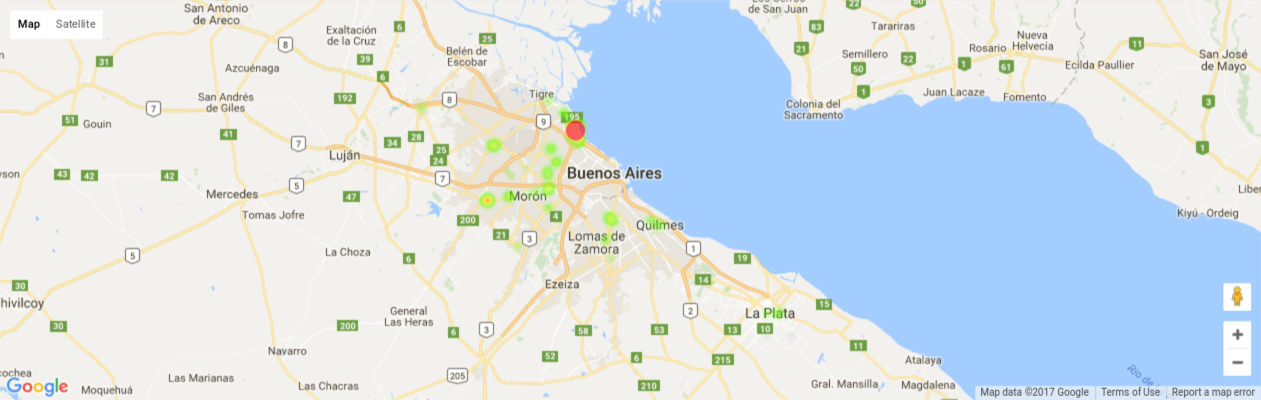
\includegraphics[width=\textwidth]{images/9}}
    				\caption{GBA con 17 instituciones}
				\end{figure}
				\FloatBarrier

				\textbf{¿Que conclusiones se obtienen de estos heatmaps?}\\	
					\tab Se pueden ubicar polos en donde hay una cantidad importante de instituciones educativas 
					(entre 17 y 20 en un rango de 400 metros de radio) y a la vez los precios por metro 
					cuadrado son altos en comparación a la totalidad de las propiedades. En ellos se 
					genera una tendencia que podría marcar una relación directa entre estos dos factores.\\ 
					Estos lugares son:
					\begin{itemize}
					\item Olivos
					\item San Cristóbal
					\item Villa Urquiza/General Urquiza
					\item Parque Patricios
					\item Colegiales
					\end{itemize}						

					A menor escala, zonas céntricas de los siguientes barrios:
					\begin{itemize}
					\item Merlo
					\item San Miguel
					\item Quilmes
					\item Recoleta
					\item Belgrano
					\item Puerto Madero
					\item Almagro
					\end{itemize}


					Resulta interesante notar una situación particular que ocurre en lugares como Villa Crespo 
					y Boedo en donde el promedio de instituciones cercanas es 9 pero sin embargo hay precios 
					muy altos en las propiedades. Esto genera una problemática en cuanto a la validez del 
					análisis por instituciones educativas y sugiere quizás realizar un filtro mas estricto 
					en los datos para futuros análisis. Sin embargo 10 instituciones educativas en un 
					rango de 400 metros sigue siendo un numero importante.\\
					
				\textbf{¿Cuales son las instituciones educativas en estos polos?}\\
					\tab A continuación se muestran los nombres de dichas instituciones por barrio
					(Solo de los 3 barrios mas significativos) para tenerlas en cuenta en 
					futuros análisis cuando se busque predecir precios por propiedades. 
					Cabe aclarar que son mas de 20 ya que se toman el conjunto de todas 
					las instituciones del barrio y no solo las de una ubicación en particular.\\
					
					\emph{\textbf{Olivos:}}
					\begin{itemize}
					\item Northlands
\item Colegio San Andrés secondary
\item Centro Cultural Italiano - Colegio Alessandro Manzoni
\item St. Andrew's Scots School
\item Instituto Jesús en el Huerto de los Olivos
\item Escuela Montessori Olivos SRL
\item Colegio San Ignacio
\item Colegio Nuestra Señora de la Paz
\item St. Luke's College
\item Action Integral Institute of Performing Arts
\item Escuela Municipal Paula Albarracín de Sarmiento
\item San Andres Secundario Olivos
\item St. Nicholas College
\item Instituto Superior De Musica Jose Hernandez
\item Escuela EPB Nº 2 “Benemérito Teniente Gral. Bartolomé Mitre”
\item UCES OLIVOS
\item Colegio Tarbut
\item Estudio Cambrée Tatiana Flaker
\item UCES UNIVERSITY OF BUSINESS AND SOCIAL SCIENCES
\item Fundacion Universidad de San Isidro
\item Colegio San Nicolas Primario
\item COLEGIO SAN NICOLAS JARDIN
\item Escuela Superior De Informatica De La Prefectura Naval Argentina
\item CENTRO PAMPA / escuela de diseño
\item Colegio Santa Magdalena
\item Colegio Eidep
\item De Los O Colegio Jesus En El Huerto
\item Jardin San Ignacio
\item E.M.P.A.S
\item Ganesha YOGA
\item Colegio Feli
\item Escuela Hija St Andrews
\item Auditorio niño Jesus De Praga
\item Escuela Municipal De Musica
\item Niño Jesús Del Praga
\item Jardín Maternal Niño Jesús de Praga
\item Auditorio Northlands School Olivos
\item Escuela De Tomas, Francisco Borges Y Rosales
\item Jardin Jho
\item Jardin de infantes CCI - Centro Cultural Italiano -
\item Jardin centro cultural italiano
\item Colegio Centro Cultural Italiano
\item SCUOLE CCI
\item Jardin Jesus en el Huerto de los Olivos
\item Jardin Dante
\item ArtBA
\item ITBA
\item Jardin Maternal Osecac
\item Instituto San Migue
\item St. Nicholas College
\item English Boutique
\item Scout Huerto De Los Olivos
\item Grupo Capoeira Brasil Buenos Aires GCB - La Lucila
\item CID vicente lopez
\item Colegio Nuestra Sra De La Paz
\item Toefl
\item Centro Cultural y Político Micaela García
\item Centro de Instrucción Aeronáutica C.I.A.
\item Escuela N 16 Marcelino Ugarte
\item Escuela EST Nro 3
					\end{itemize}				
					\emph{\textbf{San Cristóbal:}}
					\begin{itemize}
					\item DE LAS VICTORIAS
\item La Aldea del Buen Ayre
\item Instit Salesiana - Colegio San Antonio
\item Escuela Generación del Futuro
\item Danza Árabe Escuela Aldana Arguello
\item Sol de America
\item Crema y Chocolate
\item Crema y Chocolate
\item Fundacion tomas eloy martinez
\item Curso de cerrajerìa presencial e intensivo
\item Cenedi
\item AUDITORIO NAMUNCURA
\item Colegio San José de Calasanz
\item Colegio Calasanz
\item San Antonio
\item ILEC - Instituto Laico de Estudios Contemporaneos
\item Special Education Institute OUR LADY OF LUJAN
\item Curso Sublimacion
\item Escuela Domiciliaria N 2
\item JIC N 4 DE 6 MARIANO BOEDO
\item Ciber Pibes
\item Escuela Infantil Cyberpibes
\item Instructorado De KIZOMBA
\item Esc de Com Nº 22 DE 6 "G. M. Zubiria "
\item Espacio De Creacion Yapeyu
\item ESCUELA N. 6 D.E. 8 SAN JOSÉ DE CALASANZ
\item Escuela N 25 Paula A De Sarmiento
\item Pasillo al fondo "Centro Cultural"
\item Instituto Calazans
\item Escuela Lucia
\item ESCUELA PAULA ALBARRACIN DE SARMIENTO
\item Escuela Infantil La Torrecita
\item "Puente Azul" Jardín de Infantes
\item Taller De Arte Hilodearbol
\item San Antonio Salesian house
\item Curso Calidad
\item SANTA MARIA INSTITUTE
\item Instituto San Antonio-A.226
\item Escuela De TANTRACLASICO
\item CFP No.30
\item Yoga
\item Escuela No9 D.E. 8 - Florentino Ameghino
\item Supervision D E 8 Primaria
					\end{itemize}
					\emph{\textbf{Villa Urquiza/General Urquiza:}}
					\begin{itemize}
					\item School No. 24 Francisco Morazan
\item San Patricio Secondary Institute
\item Nuevos Aires SRL
\item Sir Thomas Malory
\item Mad Escuela
\item Sir Thomas Malory School
\item Estudio Joya
\item Instituto Superior del Profesorado en Educación Especial
\item INA - Instituto Nuevos Aires
\item St. Patrick's School
\item Escuela Infantil Chiquilines
\item Instituto Junín
\item The Garden of the Fund
\item Special Education School 11
\item Burdel de maderas
\item Clases de Guitarra en Villa Urquiza - Música y creatividad
\item St. Patrick's School instituto San Patricio
\item Saint Patrick
\item Acha Club
\item Caebt 56 - Parroquia Jesús Misericordioso
\item St patrick's Kinder
\item Naranon grupo
\item Escuela Nro. 4 D.E. 15
\item Escuela Nro 24 D.E.15 - Escuela Nro 8
\item Ispee
\item Facu Aye
\item Facultad Moron
\item ESc Infantil N 8 DE 15
\item San Pablo
\item Island of My Dreams
\item escuela republica de costa rica
\item Escuela No 24 SIGLO XXI
\item Escuela n•15 acevedo
\item Universidad -ciclo basico
\item Drago Uba
\item CBC Drago
\item Colegio Franco
\item UBA - Drago
\item UBA Sede Drago
\item Cbc
\item CBC UBA - Sede Drago
\item Sede Drago
					\end{itemize}
					
					Es importante notar, como se puede ver en las ultimas instituciones de 
					Villa Urquiza, la sede Drago del CBC aparece subida repetidas veces 
					pero escrita de distinta manera. Esto muestra que mas allá del gran 
					poder que tiene Google Places, los datos pueden no ser del todo fehacientes.
					
		\subsection{Análisis de la Superficie Total de la Propiedad en Metros Cuadrados} 
			A partir de este análisis se busca encontrar alguna relación entre el tamaño de la propiedad 
		y la cantidad de instituciones en su cercanía. Previo a los resultados se supone que puede 
		llegar a haber una relación teniendo en cuenta que mientras mas grande sea, es mas probable 
		que mas personas vivan allí y por consiguiente necesiten de variadas instituciones educativas. 
		A la vez se podría dar también que pequeñas propiedades estén en zonas donde la demanda de 
		instituciones educativas se muy alta y por esta razón priorizar la cercanía a las instituciones 
		dejando de lado otras comodidades como puede ser un mayor espacio.			
		
				\begin{figure}
    				\centering
    				\makebox[\textwidth]{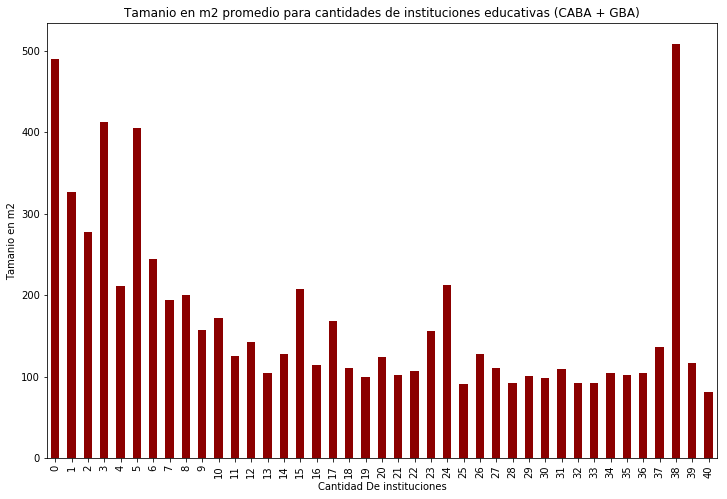
\includegraphics[width=\textwidth]{images/10}}
    				\caption{CABA + GBA}
				\end{figure}
				\begin{figure}
    				\centering
    				\makebox[\textwidth]{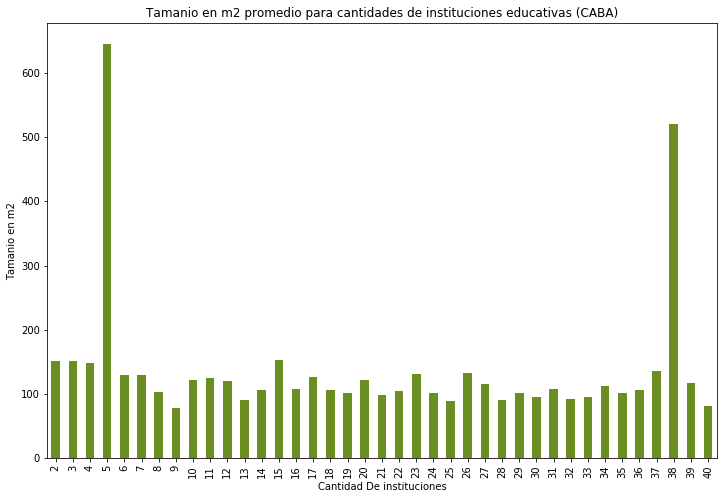
\includegraphics[width=\textwidth]{images/11}}
    				\caption{CABA}
				\end{figure}
				\begin{figure}
    				\centering
    				\makebox[\textwidth]{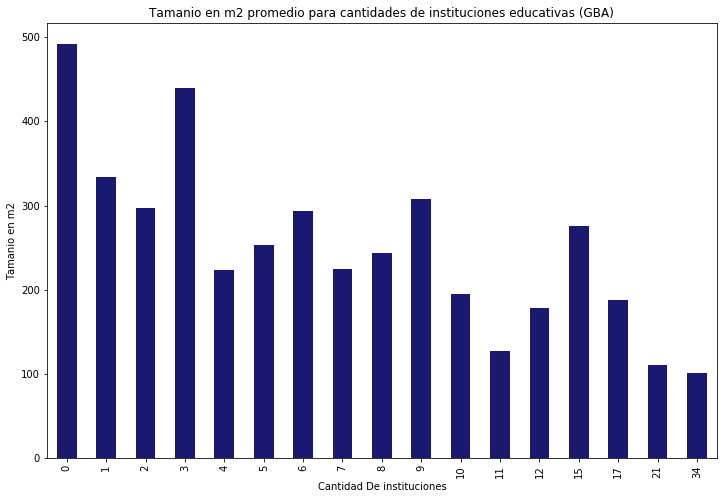
\includegraphics[width=\textwidth]{images/12}}
    				\caption{GBA}
				\end{figure}
				\FloatBarrier
				
				Al darle una vista rápida a los gráficos se  ven que los comportamientos de 
				CABA Y GBA son muy distintos. Pero en este caso los picos máximos tienen 
				valores similares rondando entre 500 y 600 metros cuadrados. 
				Se procede a analizar los datos por separado para obtener conclusiones mas precisas.\\
				
				\textbf{¿Que conclusiones se obtienen de GBA?}\\
				En GBA se ve una tendencia a la baja de tamaños, siendo que a mayor 
				cantidad de instituciones, las propiedades tienen un tamaño menor. 
				Una posible razón puede adjudicarse a que muchas de las propiedades 
				de GBA pertenecientes al Dataframe son de barrios cerrados en donde 
				los terrenos suelen ser particularmente grandes y a la vez las 
				distancias a, no solo instituciones educativas si no también a 
				locales o zonas con mayor población, son superiores.\\
				
				\textbf{Relación entre el tamaño total de la superficie y la cantidad de 
				instituciones educativas para CABA}\\
				Se distinguen dos claros picos máximos en 5 instituciones, y en 38. 
				Mas allá de esto no se ven otras relaciones que resulten de interés 
				para el análisis. Para ubicar las propiedades en cuestión se realiza 
				un heapmap con ellas.
					
				\begin{figure}
    				\centering
    				\textbf{HEATMAP por ubicaciones}\par\medskip
    				\makebox[\textwidth]{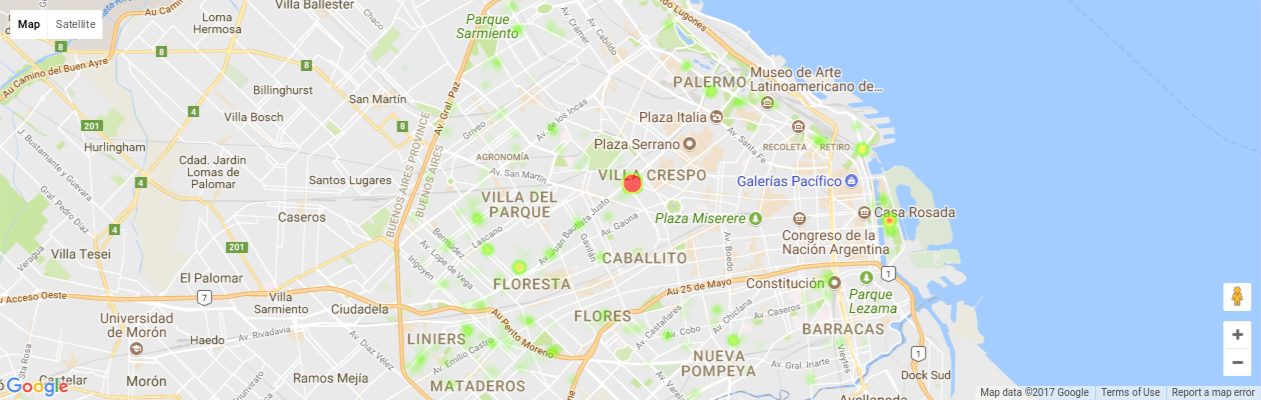
\includegraphics[width=\textwidth]{images/13}}
    				\caption{CABA con 5 instituciones}
				\end{figure}				
				\begin{figure}
    				\centering
    				\textbf{HEATMAP por tamaño de superficie}\par\medskip
    				\makebox[\textwidth]{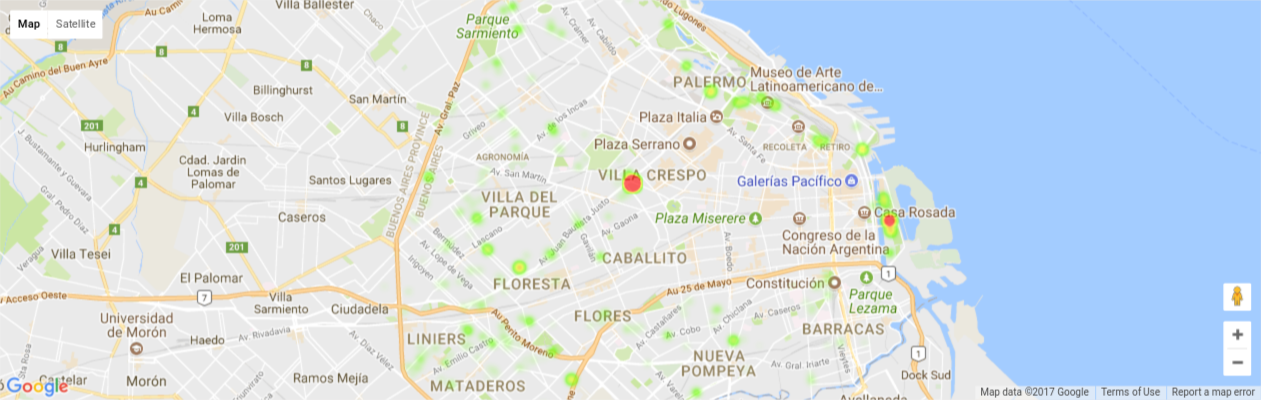
\includegraphics[width=\textwidth]{images/14}}
    				\caption{CABA con 5 instituciones}
				\end{figure}				
				\begin{figure}
    				\centering
    				\textbf{HEATMAP por ubicaciones}\par\medskip
    				\makebox[\textwidth]{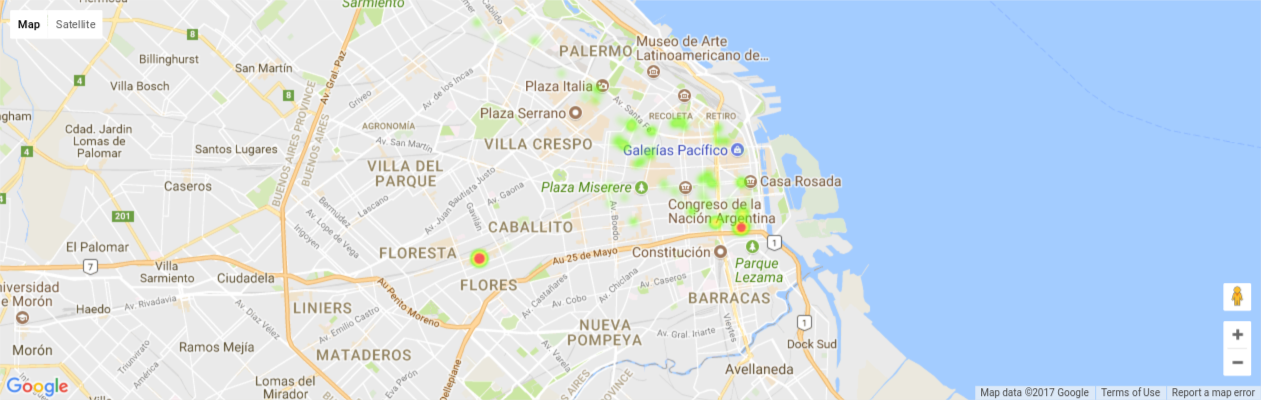
\includegraphics[width=\textwidth]{images/15}}
    				\caption{CABA con 38 instituciones}
				\end{figure}				
				\begin{figure}
    				\centering
    				\textbf{HEATMAP por tamaño de superficie}\par\medskip
    				\makebox[\textwidth]{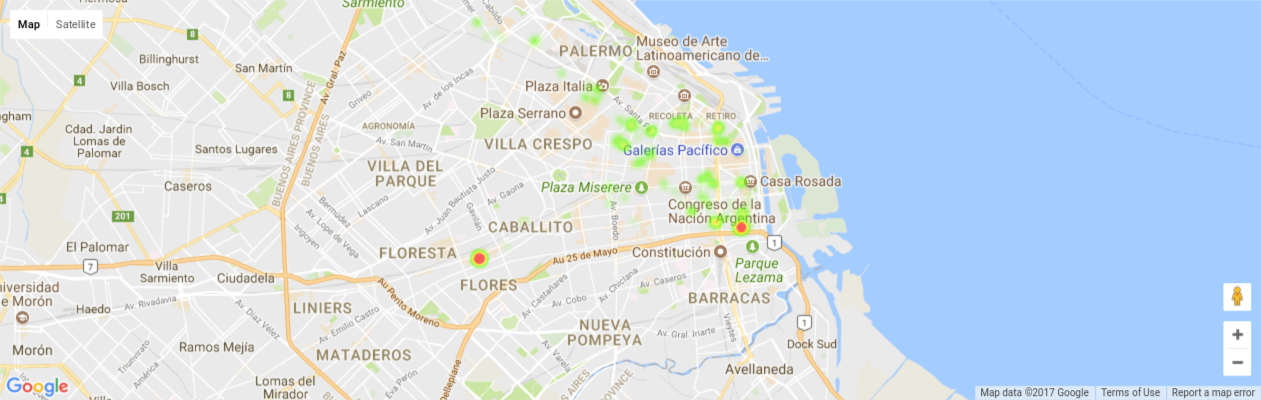
\includegraphics[width=\textwidth]{images/16}}
    				\caption{CABA con 38 instituciones}
				\end{figure}				
				\FloatBarrier
				
				\textbf{¿Que conclusiones se obtienen de estos heatmaps?}\\
				En los heatmaps con 5 propiedades en CABA se marca la tendencia que ubicaba a 
				Villa Crespo como un polo. En donde hay una base solida pero no muy grande de 
				instituciones educativas y a la vez hay precios altos por metro cuadrado y 
				propiedades de tamaños importantes. A esto se agrega la zona de puerto madero 
				en donde se observan precios muy altos, grandes propiedades, y un buen numero 
				de instituciones educativas, particularmente universidades.\\
				Finalmente se ubican dos nuevos polos con propiedades muy grandes y realmente un numero 
				enorme de instituciones (38 instituciones) siendo estos Plaza Dorrego y en Flores cerca 
				de la Av. Rivadavia entre Av.Nazca y Av.Carabobo.
		\section{Análisis de Locales Gastronómicos}
			\emph{A continuación se encuentra el análisis de las instituciones de tipo gastronómicas para 
			un set de datos completo de 72474 entradas.}
			\subsection{Análisis del precio por metro cuadrado}
				Para los siguientes gráficos se agruparon las propiedades por cantidad de instituciones 
				cercanas y sacando el promedio del precio por metro cuadrado para ellas. 
				Para que los resultados sean significativos, se filtro a todas los conjuntos 
				de propiedades con un precio menor a \textdollar USD8000 teniendo en cuenta 
				el análisis inicial.
				
				\begin{figure}
    				\centering
    				\makebox[\textwidth]{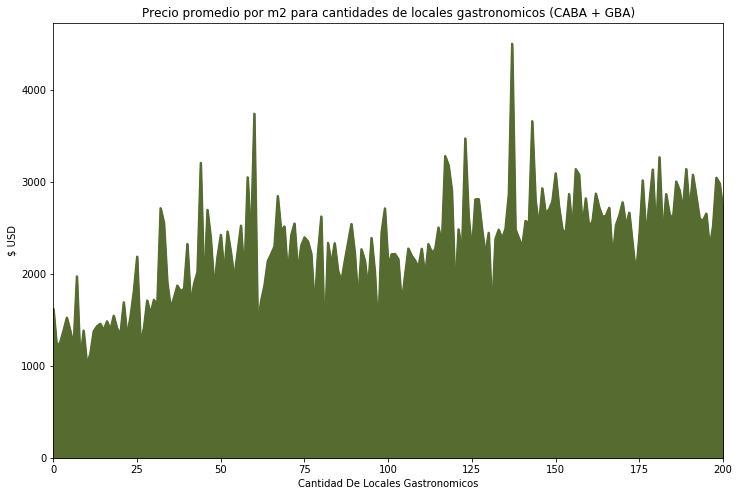
\includegraphics[width=\textwidth]{images/17}}
    				\caption{CABA + GBA}
				\end{figure}
				\begin{figure}
    				\centering
    				\makebox[\textwidth]{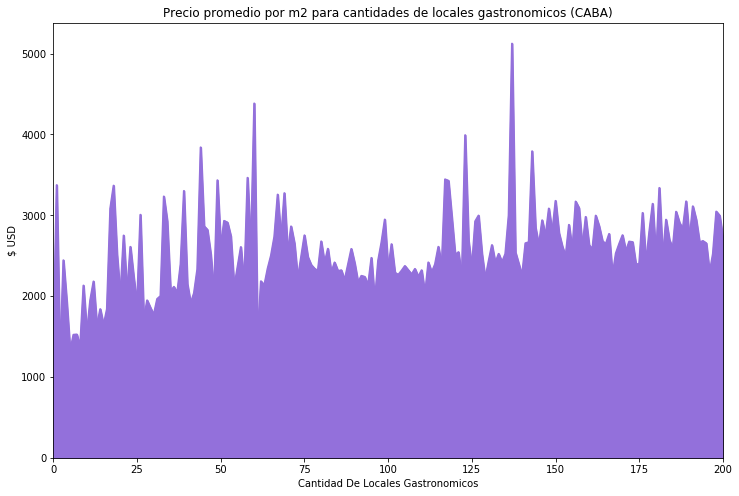
\includegraphics[width=\textwidth]{images/18}}
    				\caption{CABA}
				\end{figure}
				\begin{figure}
    				\centering
    				\makebox[\textwidth]{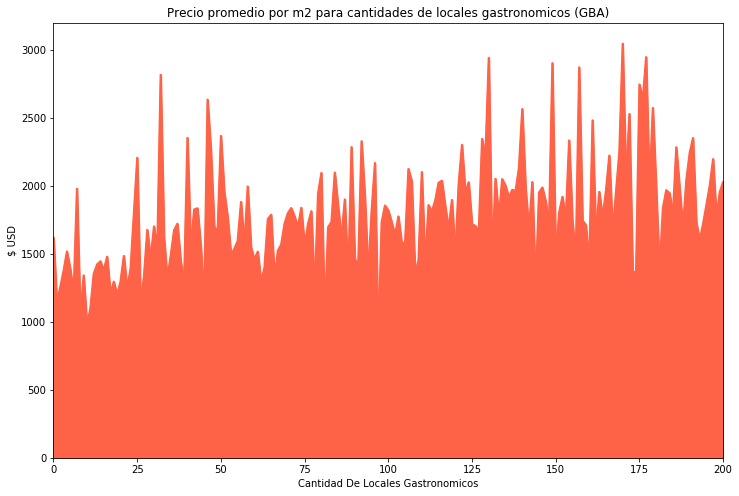
\includegraphics[width=\textwidth]{images/19}}
    				\caption{GBA}
				\end{figure}
				\FloatBarrier
				
				A simple vista los gráficos no dicen mucho. Es observable una leve tendencia de 
				crecimiento en cuanto a mayor cantidad de locales el precio de las propiedades 
				seria mayor y lo mismo para menor cantidad de locales. Dicha tendencia se puede 
				apreciar mejor en el gráfico de GBA + CABA. En los otros gráficos, la tendencia 
				de punta a punta (mas allá de abruptas variaciones) se asemeja a constante.  
				Se procede a ubicar donde están los lugares con menores locales y donde están 
				los que mas tienen, es decir, los extremos.
				
				\begin{figure}
    				\centering
    				\textbf{Heatmap con el peso en el precio por metro cuadrado de locales gastronómicos}\par\medskip
    				\makebox[\textwidth]{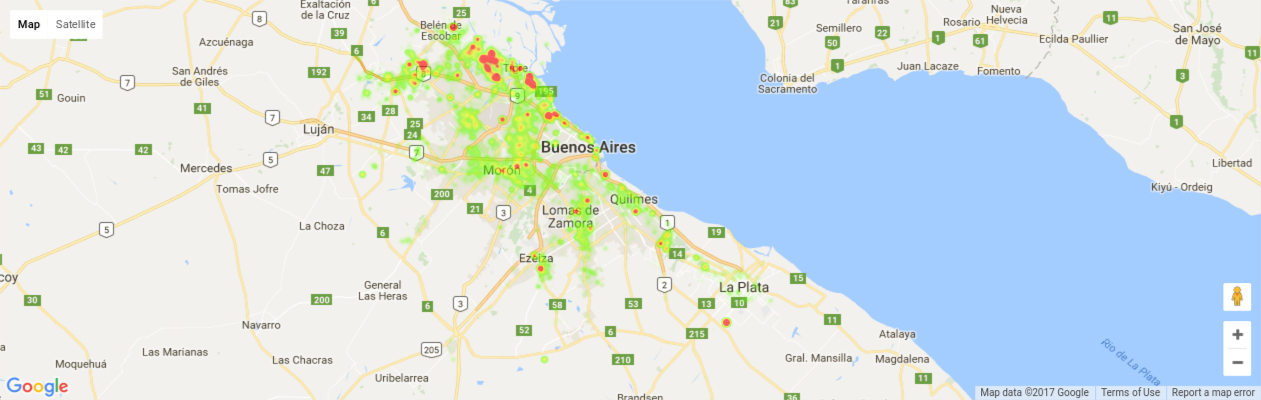
\includegraphics[width=\textwidth]{images/20}}
    				\caption{CABA + GBA de 0 a 20 locales}
				\end{figure}				
				\begin{figure}
    				\centering
    				\textbf{Mismo Heatmap que la figura anterior pero con ZOOM}\par\medskip
    				\makebox[\textwidth]{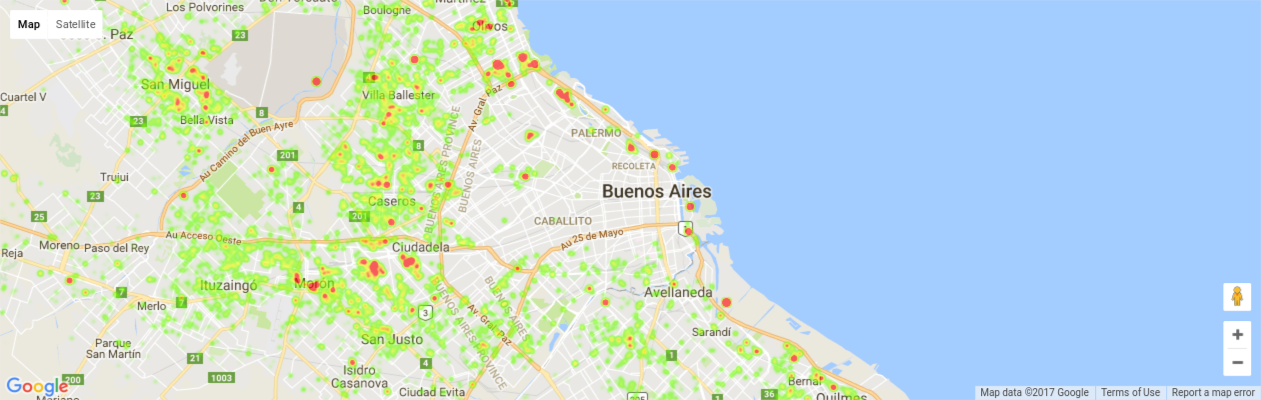
\includegraphics[width=\textwidth]{images/21}}
    				\caption{CABA + GBA de 0 a 20 locales}
				\end{figure}
				\FloatBarrier				
				
				De estos últimos heatmaps se puede extraer la interesante conclusión de que 
				las propiedades con pocos locales gastronómicos a su alrededor pertenecen a 
				GBA y prácticamente excluyen a CABA.				
								
				\begin{figure}
    				\centering
    				\textbf{Heatmap con el peso en el precio por metro cuadrado de locales gastronómicos}\par\medskip
    				\makebox[\textwidth]{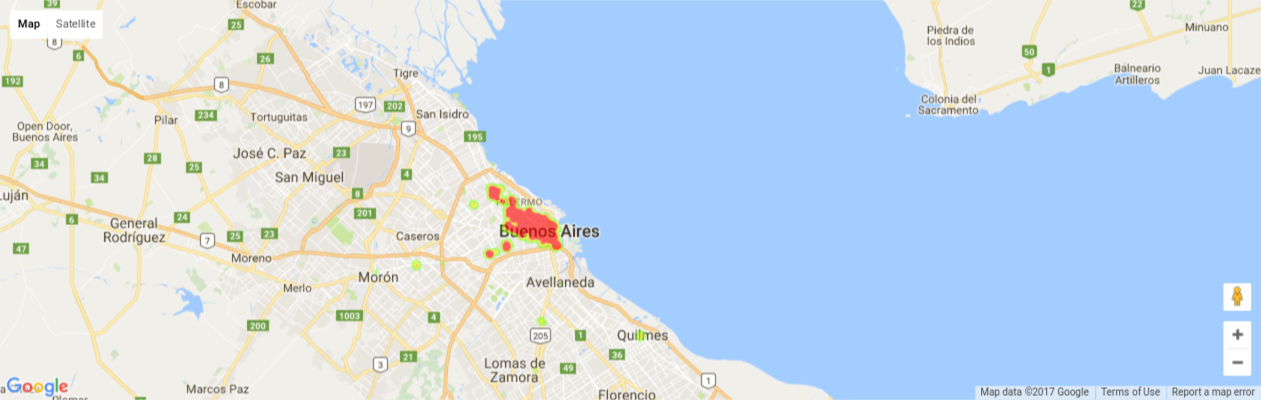
\includegraphics[width=\textwidth]{images/22}}
    				\caption{CABA + GBA de 180 a 200 locales}
				\end{figure}								
				\FloatBarrier
				
				Continuando con el análisis previo, las propiedades con entre 180 y 200 
				locales gastronómicos en sus cercanías están en su totalidad ubicados en CABA, 
				mas particularmente su zona céntrica.\\
				
				\textbf{Principales polos gastronómicos}\\
				Analizando mas detalladamente las posiciones de las propiedades 
				en el mapa se encuentran los siguientes sectores como principales polos gastronómicos:
\begin{itemize}
	\item Plaza Serrano
	\item Recoleta
	\item Plaza Dorrego
	\item Belgrano
\end{itemize}


				Cabe aclara que en GBA las mayores concentraciones están ubicadas en la 
				cercanía de centros comerciales (shopping centers).
	
		\section{Análisis de Puntos de Interés Cultural}
			\emph{A continuación se encuentra el análisis de los puntos de interés cultural 
			para un set de datos completo de 72474 entradas.}
			
			\subsection{Análisis del precio por metro cuadrado}
				Primero se comienza sin agregar ningún recorte extra al set de datos y se 
				analiza una descripción del set de datos. Utilizando la función describe, 
				es posible notar que menos del \%50 de los datos tienen una cantidad de 
				entradas menor a 60. Esto quiero decir que puede haber por ejemplo solo 
				una propiedad con un numero muy alto de entradas que distorsiones a todo 
				el resto. Como lo que se esta tratando de buscar son tendencias. 
				Se procede a cortar la cantidad de instituciones por el porcentual del \%99 
				para achicar posibles disrupciones. 
				Finalmente recortando por cantidad de puntos culturales menores a 65 y 
				que estos tengan por lo menos 10 repeticiones se obtienen los siguientes gráficos:

				\begin{figure}
    				\centering
    				\makebox[\textwidth]{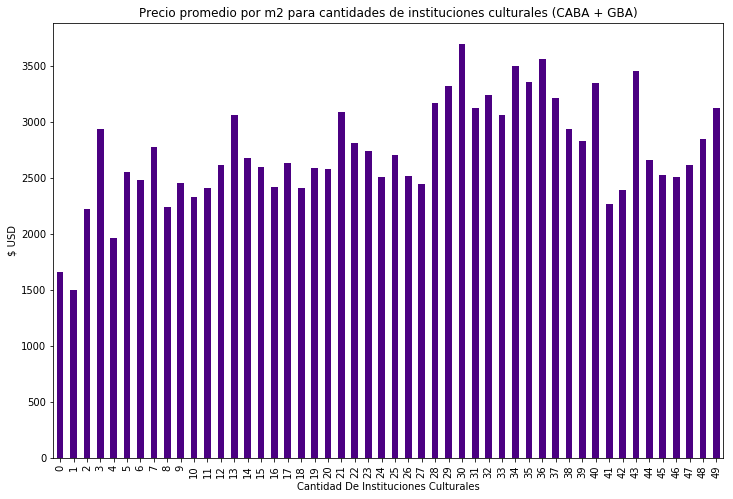
\includegraphics[width=\textwidth]{images/23}}
    				\caption{CABA + GBA}
				\end{figure}
				\begin{figure}
    				\centering
    				\makebox[\textwidth]{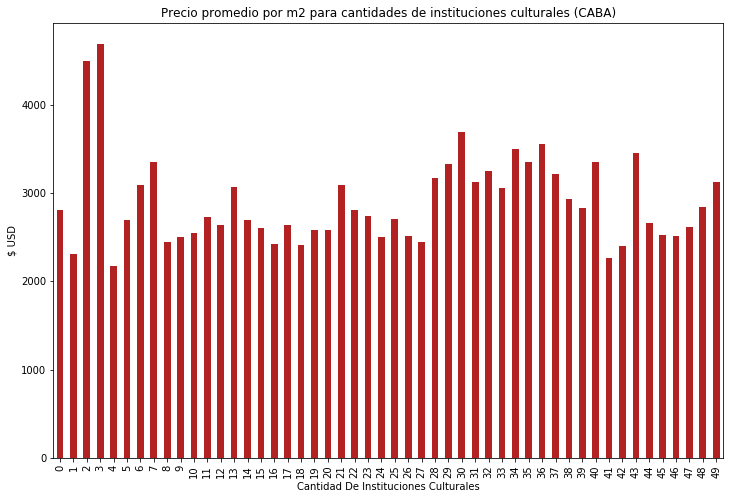
\includegraphics[width=\textwidth]{images/24}}
    				\caption{CABA}
				\end{figure}
				\begin{figure}
    				\centering
    				\makebox[\textwidth]{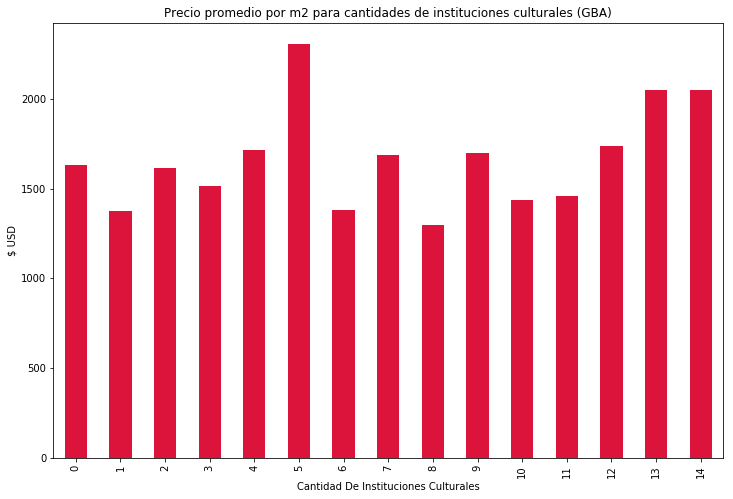
\includegraphics[width=\textwidth]{images/25}}
    				\caption{GBA}
				\end{figure}
				\FloatBarrier
				
				Instantáneamente se percibe lo que conociendo el territorio seria sospechable. 
				Esto es en primer medida que la cantidad de puntos de interés cultural en 
				CABA contra los de GBA es considerablemente mayor siendo 49 contra 14 las 
				respectivas cantidades máximas. A la vez es notable resaltar que en gráfico 
				de CABA + GBA hay una clara disminución en el precio de la propiedad para 
				lugares con 0 o 1 puntos cercanos. Mas allá de estos conceptos, los tendencias 
				sugieren ser a simple vista constantes.\\ 
				\tab Se trata de ubicar a las propiedades con pocos puntos cercanos en zonas particulares.						 					
				\begin{figure}
    				\centering
    				\textbf{Heatmap con el peso en las ubicaciones}\par\medskip
    				\makebox[\textwidth]{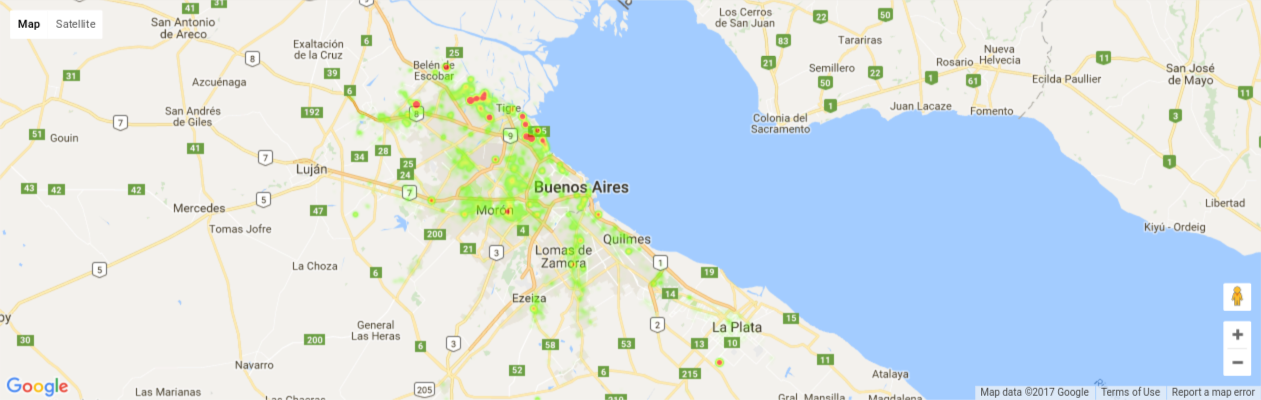
\includegraphics[width=\textwidth]{images/26}}
    				\caption{CABA + GBA con 0 o 1 puntos de interés cultural cerca}
				\end{figure}				
				\FloatBarrier
				
				Como los gráficos anticipaban, casi en su totalidad estas propiedades están ubicadas en GBA. 
				Sin embargo surge un punto interesante y es que se concentran mas que nada en la zona 
				norte de GBA. Esto podría adjudicarse a que un gran porcentaje de las propiedades 
				utilizadas pertenecen efectivamente a esa zona.\\ 

				Al tratar de analizar los gráficos previos, los diferenciados por CABA 
				muestran indicios de que podría aplicarse una análisis mas particular para 
				lograr obtener sus polos mas importantes como se realizo con el resto de las 
				investigaciones. Es así que se realiza un nuevo gráfico pero esta vez 
				recortando a las cantidades de puntos de interés con bajas frecuencias, 
				para así encontrar concentraciones mas importantes.	
				
				\begin{figure}
    				\centering
    				\makebox[\textwidth]{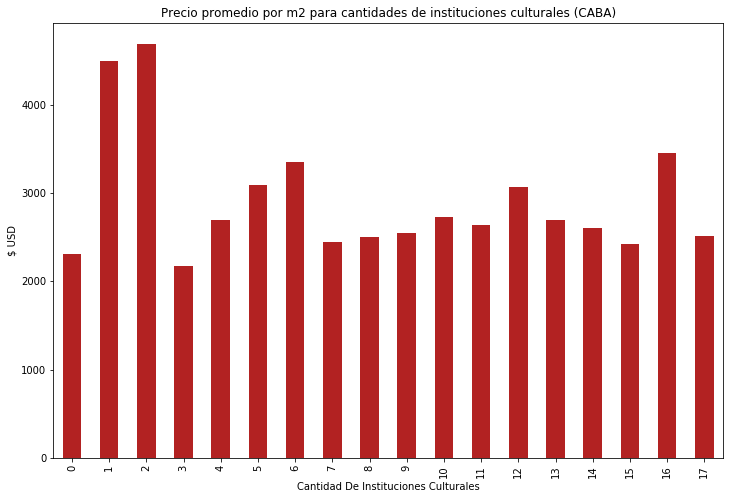
\includegraphics[width=\textwidth]{images/27}}
    				\caption{CABA}
				\end{figure}
				\FloatBarrier
				
				Los picos en 1 y 2 instituciones se siguen sosteniendo mas allá de la filtración de 
				los datos, esto podría sugerir o que la gran mayoría de las propiedades en CABA 
				tienen esa cantidad de instituciones cerca, o algo mas difícil de demostrar que 
				quizás tener pocas instituciones cerca realmente mejora el precio de la propiedad.\\
				\tab Se asilan los puntos en CABA con una o dos instituciones cerca y se las ubica en un heatmap.
				
				\begin{figure}
    				\centering
    				\textbf{Heatmap con el peso en las ubicaciones}\par\medskip
    				\makebox[\textwidth]{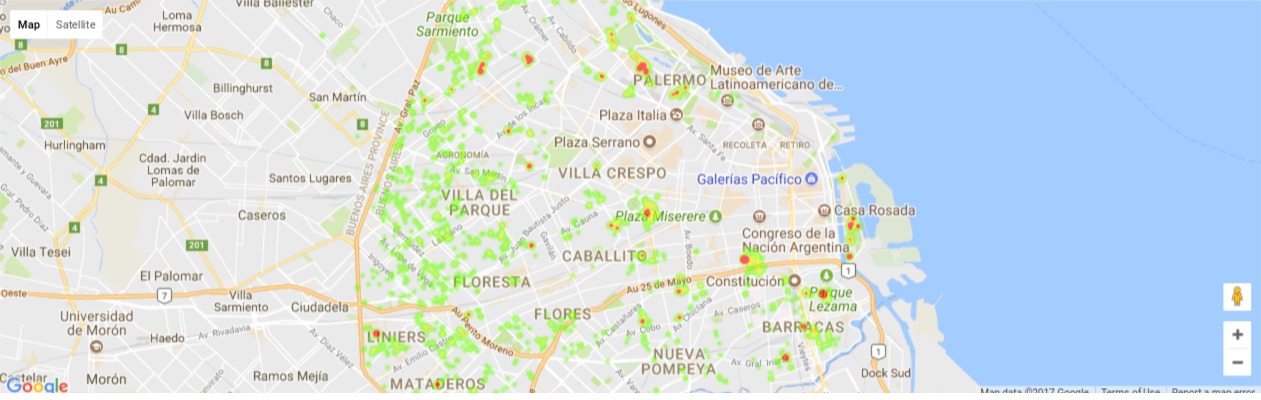
\includegraphics[width=\textwidth]{images/28}}
    				\caption{CABA  con 2 o 3 puntos de interés cultural cerca}
				\end{figure}				
				\FloatBarrier
				
				Las propiedades en cuestión están ubicadas en las periferias de la zona céntrica de CABA  
				(salvo excepciones). Esto muestra que hay un numero de propiedades con un valor alto 
				por metro cuadrado que se ubican lejos de las zonas con mas afluencia de personas, 
				o hasta turistas, ya que los puntos de interés culturales suelen ser visitados por 
				ellos. Esto podría sugerir que al estar “aislado” de los lugares mas transitados 
				pero seguir perteneciendo a la capital le da un valor elevado a la propiedad, 
				mas que nada en el sentido de lugares de residencia.\\
				
				\textbf{Principales polos de puntos de interés cultural}
				
				\begin{figure}
    				\centering
    				\textbf{Heatmap con el peso en la cantidad de puntos de interés cultural cercanos}\par\medskip
    				\makebox[\textwidth]{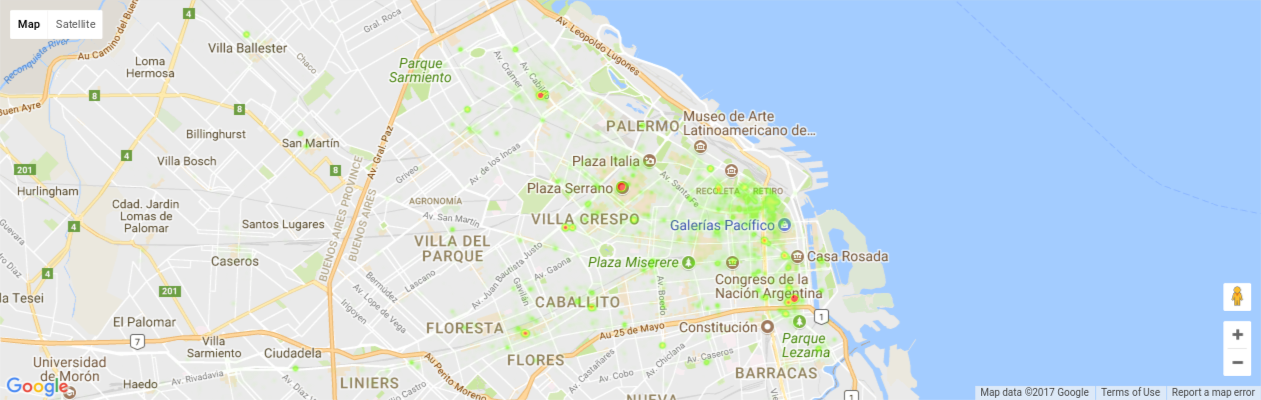
\includegraphics[width=\textwidth]{images/29}}
    				\caption{CABA propiedades con mayor cantidad puntos de interés cultural cerca}
				\end{figure}				
				\FloatBarrier
				
				Analizando mas detalladamente las posiciones de las propiedades en el mapa se encuentran 
				los siguientes sectores como principales polos de lugares culturales:
				
				\begin{itemize}
					\item Plaza Serrano
					\item Plaza Dorrego
					\item Belgrano
				\end{itemize}

				Es interesante comparar estos resultados con los polos gastronómicos. 
				Parecería que al menos a simple vista hay una correlación entre los 
				ambos puntos con mayor concentración de puntos de interés cultural y de locales gastronómicos. 
		
		\section{Análisis de Transporte Publico}
			\emph{A continuación se encuentra el análisis de los servicios de transporte publico para un 
			set de datos completo de 72474 entradas.\\
			Con transporte publico se refiere a las paradas o estaciones de colectivos o 
			subterráneos en un radio de 400m de la propiedad.} 												
			\subsection{Análisis del precio por metro cuadrado}
				Para los siguientes gráficos se agruparon las propiedades por cantidad de paradas de 
				transporte publico cercanas y sacando el promedio del precio por metro cuadrado para 
				ellas. Al ser el máximo de 57 paradas relativamente bajo para el radio tomado, 
				se filtro a todas los conjuntos de propiedades con menos de 10 entradas para las 
				cantidades de paradas cercanas y así levemente limpiar de distorsión al set de datos.
				 		
				\begin{figure}
    				\centering
    				\makebox[\textwidth]{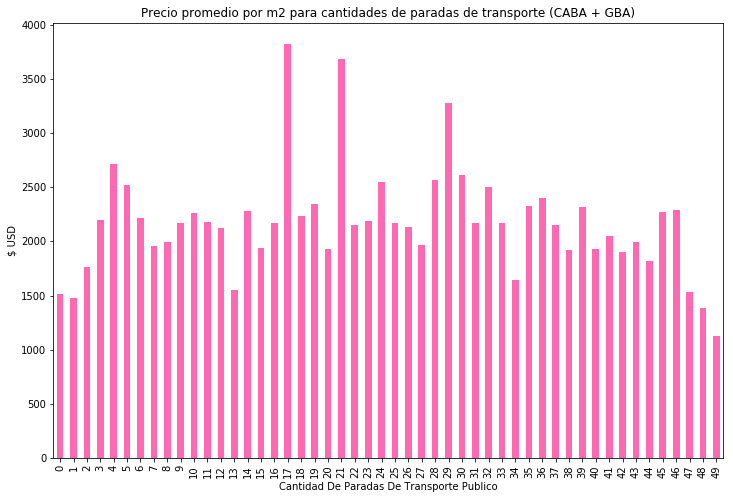
\includegraphics[width=\textwidth]{images/30}}
    				\caption{CABA + GBA}
				\end{figure}
				\begin{figure}
    				\centering
    				\makebox[\textwidth]{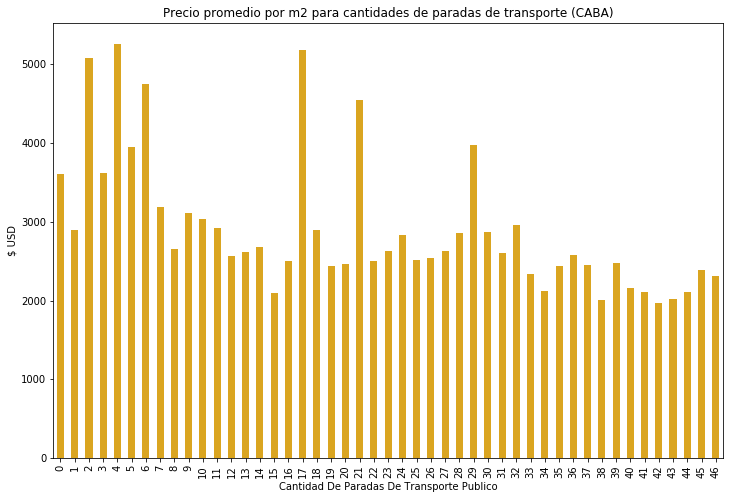
\includegraphics[width=\textwidth]{images/31}}
    				\caption{CABA}
				\end{figure}
				\begin{figure}
    				\centering
    				\makebox[\textwidth]{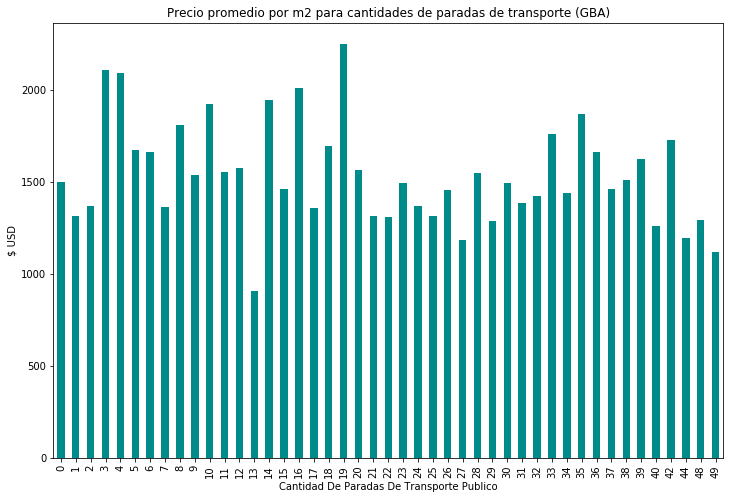
\includegraphics[width=\textwidth]{images/32}}
    				\caption{GBA}
				\end{figure}
				\FloatBarrier
				
				Analizando el gráfico que contempla GBA + CABA se puede ver una especie de campana en donde 
				los menores precios por metro cuadrado estarían concentrados en los extremos y en el centro 
				los picos mayores. Este tendencia sin embargo no se sostiene en el resto. En CABA parecería 
				ser como hay un leve decaimiento en el precio a medida que aumenta la cantidad de paradas. 
				Nuevamente los máximos de CABA y GBA son significativamente distintos, siendo casi la mitad 
				el de GBA. Se continua analizando las distintas anomalías o tendencias recién mencionadas 
				para encontrar patrones.\\
				
				\textbf{Separación de CABA + GBA por precio}\\
				\tab\textdollar USD2000 por metro cuadrado parecería ser una linea prudente por la cual 
				dividir las propiedades y analizar la distribución en la cantidad de paradas. 

				\begin{figure}
    				\centering
    				\textbf{Heatmap con el peso puesto en la cantidad de paradas}\par\medskip
    				\makebox[\textwidth]{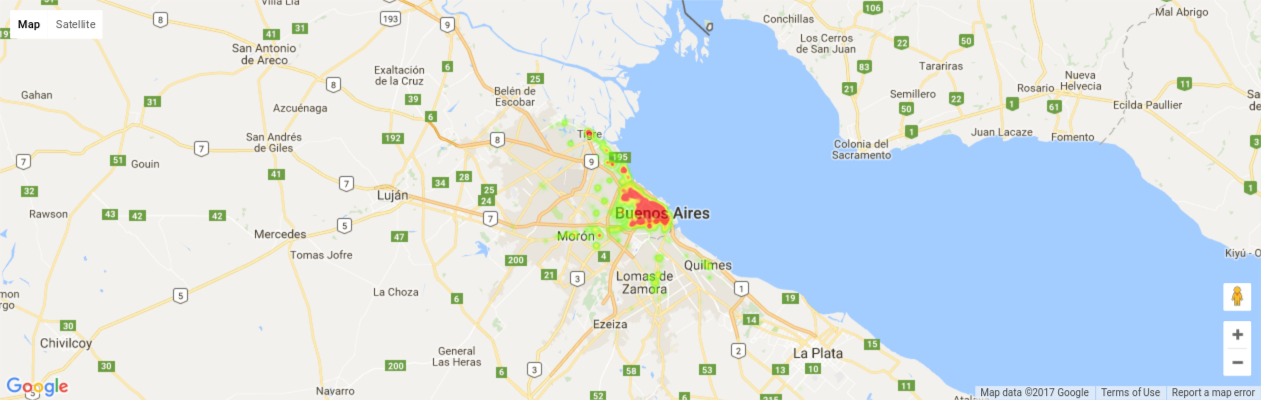
\includegraphics[width=\textwidth]{images/33}}
    				\caption{CABA + GBA propiedades con precio por metro cuadrado mayor a \textdollar USD2000}
				\end{figure}
				\begin{figure}
    				\centering
    				\textbf{Zoom de la figura anterior}\par\medskip
    				\makebox[\textwidth]{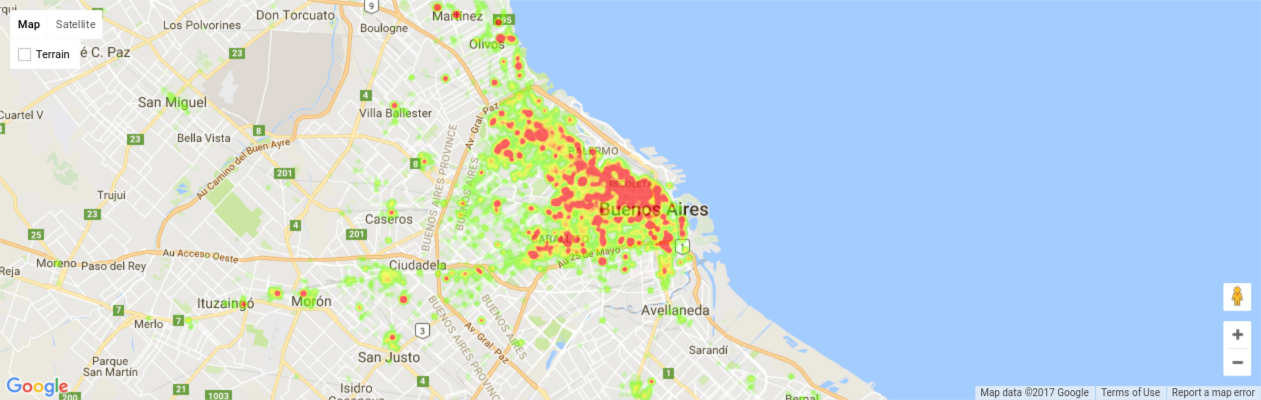
\includegraphics[width=\textwidth]{images/34}}
    				\caption{CABA + GBA propiedades con precio por metro cuadrado mayor a \textdollar USD2000}
				\end{figure}								
				\FloatBarrier
				
				Hay una clara concentración en la capital, con la excepción de centros de los cordones mas 
				inmediatos de GBA. Viendo el siguiente mapa de trenes y subterráneos, este muestra como 
				el tendido de redes se expande a medida que uno se aleja del centro de CABA. El heatmap 
				parecería tener una forma muy similar sugiriendo que las propiedades de mayor precio 
				podrían estar situadas cerca de paradas de subterráneo. Teniendo en cuenta que la 
				distribución de paradas de colectivos por la capital es mas pareja, esto apoyaría a 
				la hipótesis planteada.
				
				\begin{figure}
    				\centering
    				\makebox[\textwidth]{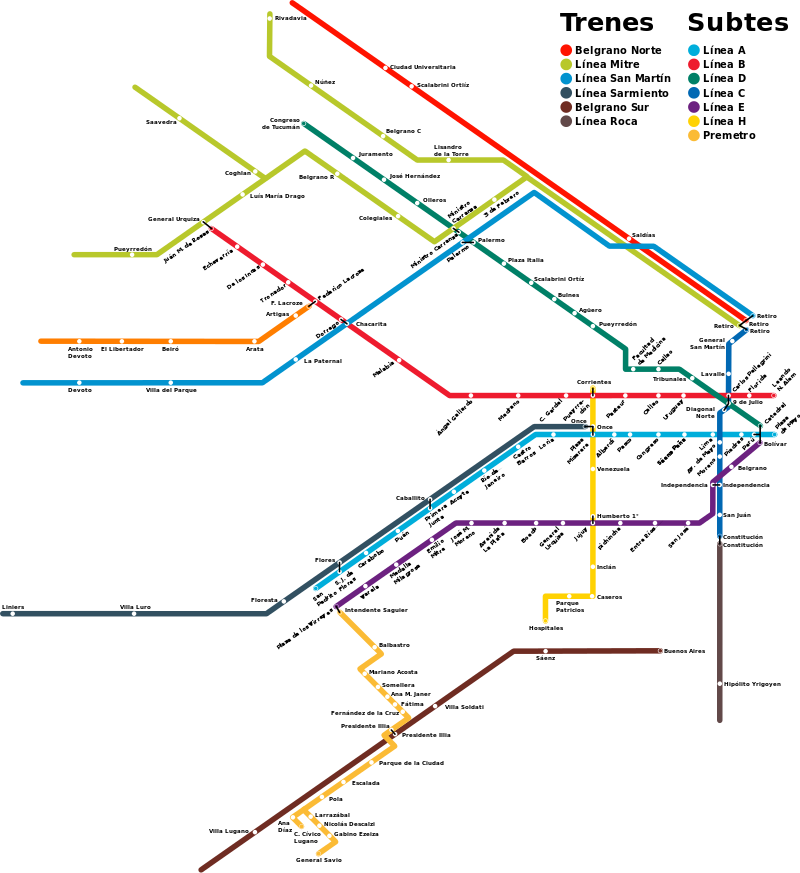
\includegraphics[width=\textwidth]{images/35}}
    				\caption{Red de Subterraneos y Trenes de Buenos Aires}
				\end{figure}
				\begin{figure}
    				\centering
    				\textbf{Heatmap con el peso puesto en la cantidad de paradas}\par\medskip
    				\makebox[\textwidth]{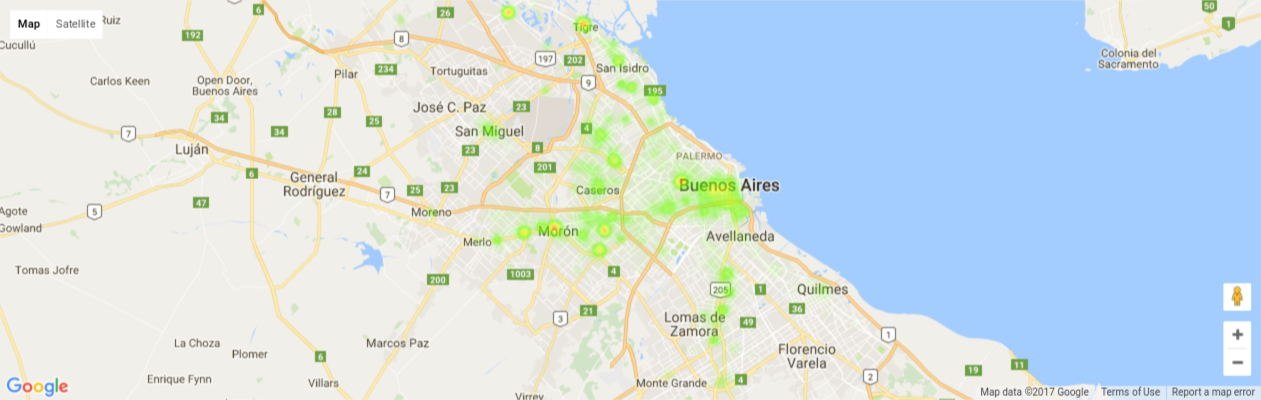
\includegraphics[width=\textwidth]{images/36}}
    				\caption{CABA + GBA propiedades con precio por metro cuadrado menor a \textdollar USD2000}
				\end{figure}
				\FloatBarrier
				
				La cantidad de propiedades menores a \textdollar USD2000 parecerían ser las de menor 
				cantidad de paradas de transporte publico cercanas. Eso se denota ya que los heatmaps 
				están armados utilizando como peso la cantidad de paradas cercanas. Es decir que 
				mientras mas paradas cercanas tenga, mas roja se vera la ubicación en el mapa. 
				A la vez se ve que las concentraciones de lugares con muchas paradas se ubican en 
				las principales zonas de GBA (a nivel de población) siendo estas Morón, 
				San Miguel, Tigre, Lomas de Zamora, entre otras.\\
				
				\textbf{Zonas de CABA + GBA por mayor cantidad de paradas}\\
				Se ubican las propiedades con mas de 35 paradas de transporte publico cercanas.
				
				\begin{figure}
    				\centering
    				\textbf{Heatmap con el peso puesto en la cantidad de paradas}\par\medskip
    				\makebox[\textwidth]{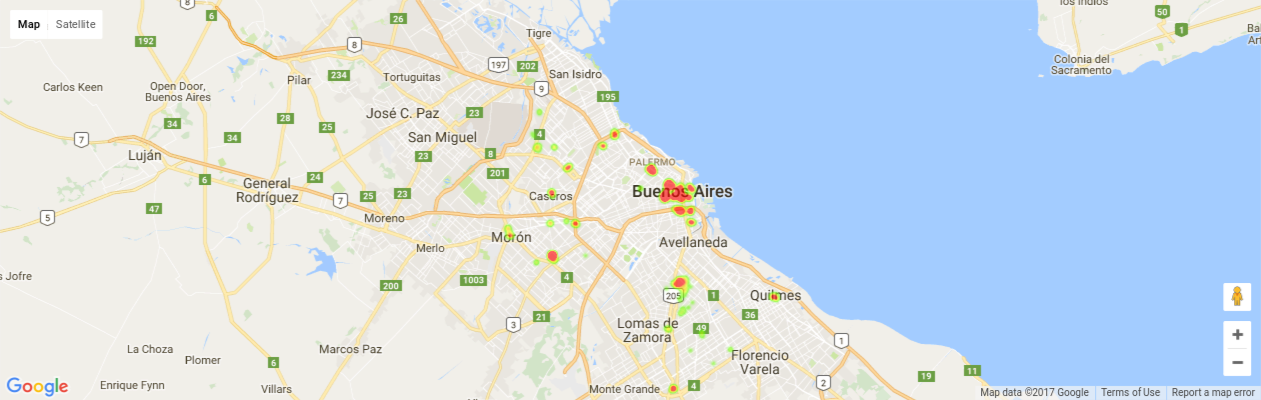
\includegraphics[width=\textwidth]{images/37}}
    				\caption{CABA + GBA propiedades con mas de 35 paradas cerca}
				\end{figure}
				\FloatBarrier				
				
				Gran parte de estos pertenecen al microcentro de CABA, mientras que a la vez se 
				encuentran ciertos puntos con una alto concentracion:
				\begin{itemize}
					\item Lanus
					\item San Justo
					\item Constitucion
					\item Quilmes
				\end{itemize}
				\begin{figure}
    				\centering
    				\textbf{Heatmap anterior con ZOOM en CABA}\par\medskip
    				\makebox[\textwidth]{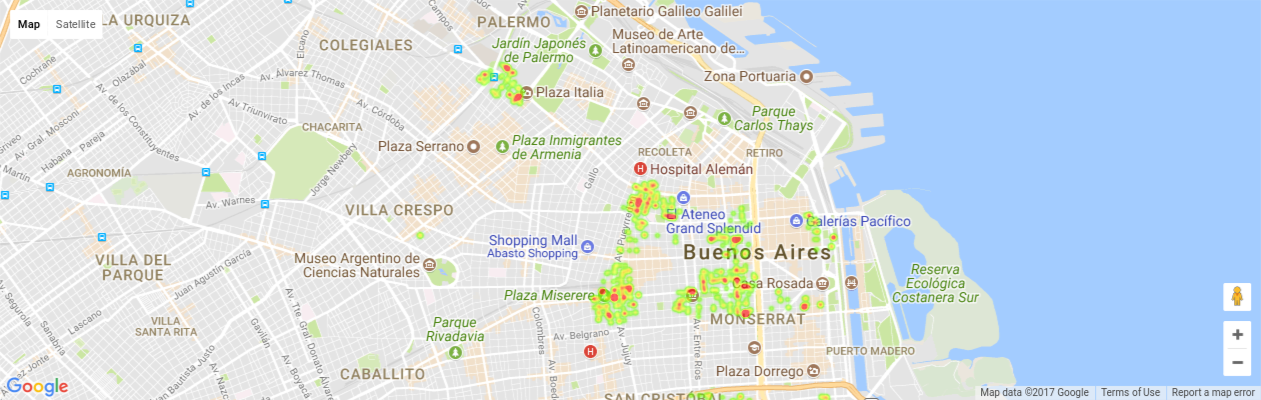
\includegraphics[width=\textwidth]{images/38}}
    				\caption{CABA propiedades con mas de 35 paradas cerca}
				\end{figure}

				\FloatBarrier
				
				Lógicamente, las propiedades con mayor cantidad de paradas cercanas se encuentran en el 
				micro-centro porteño, de donde salen todas las lineas de subterráneo y una abundante 
				cantidad de colectivos. A la vez Plaza Italia, Plaza Miserere y la zona de la Facultad 
				de Medicina funcionan como puntos principales.\\				
				
				\textbf{Zonas de CABA + GBA por menor cantidad de paradas}\\
				Se ubican las propiedades con 7 o menos paradas de transporte publico cercanas. 
				(Heatmap con el peso en la cantidad de paradas)
				
				\begin{figure}
    				\centering
    				\textbf{Heatmap con el peso en la cantidad de paradas}\par\medskip
    				\makebox[\textwidth]{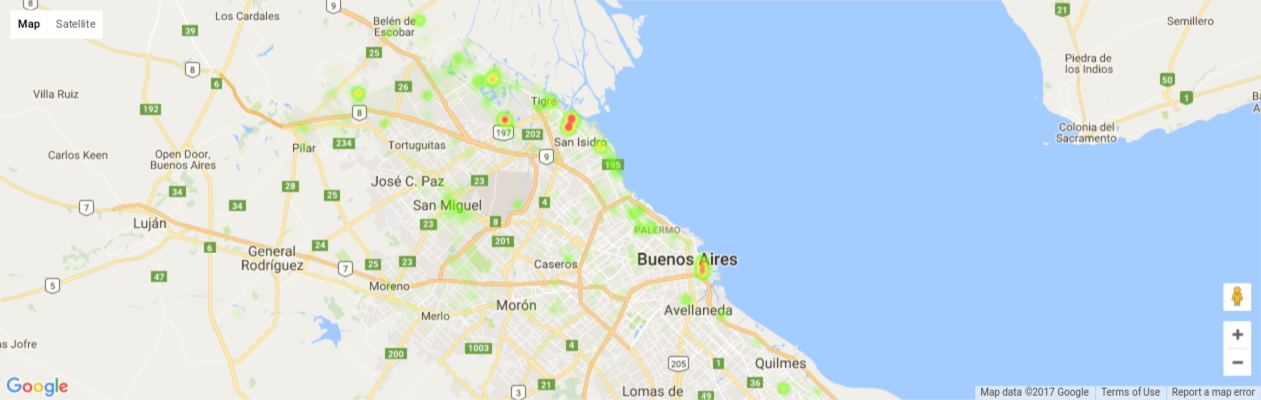
\includegraphics[width=\textwidth]{images/39}}
    				\caption{CABA propiedades con 7 o menos paradas de transporte publico cercanas}
				\end{figure}
				\FloatBarrier
				
				El Heatmap permite rápidamente identificar a Puerto Madero, Tigre, Pacheco y parte de 
				San Isidro como lugares en donde hay una reducida cantidad de paradas de transporte 
				publico en comparación al resto del territorio.\\ 

				\textbf{Distribución de las cantidad de paradas contra el precio por metro cuadrado en CABA (desarrollo de hipótesis de red de transporte)}\\
				
				El siguiente mapa muestra el tendido de las redes subterráneas por la ciudad de Buenos Aires siendo:
				\begin{itemize}
					\item Linea A (Celeste)
					\item Linea B (Roja)
					\item Linea C (Azul)
					\item Linea D (Verde)
					\item Linea E (Violeta)
					\item Linea H (Amarilla)
				\end{itemize}
			
				\begin{figure}
    				\centering
    				\makebox[\textwidth]{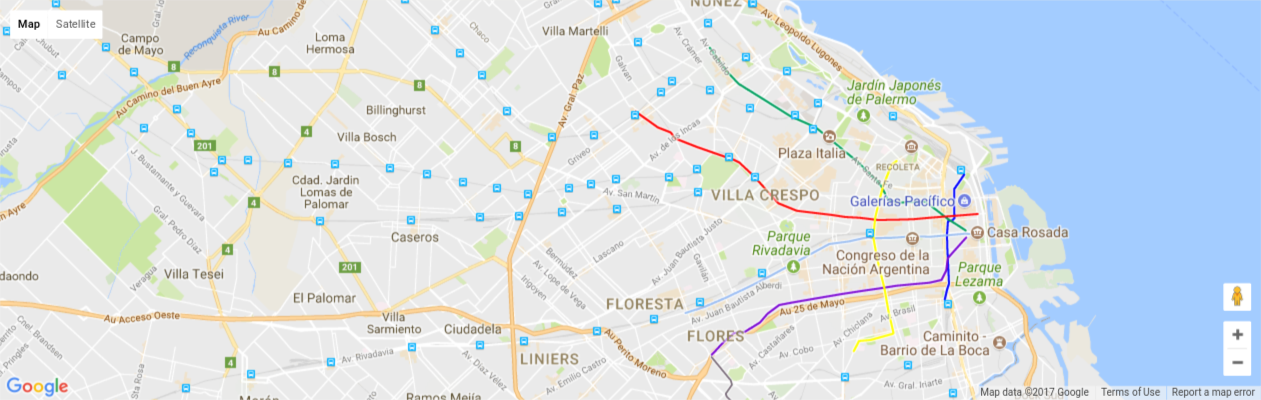
\includegraphics[width=\textwidth]{images/40}}
    				\caption{Red de Subterraneos Buenos Aires}
				\end{figure}
				\FloatBarrier
				
				Teniendo en cuenta dicho tendido se procede a graficar en un heapmap el conjunto de propiedades 
				(CABA + GBA) teniendo en cuenta como peso del Heatmap la cantidad de paradas cercanas.
			
				\begin{figure}
    				\centering
    				\textbf{Heatmap con el peso en la cantidad de paradas}\par\medskip
    				\makebox[\textwidth]{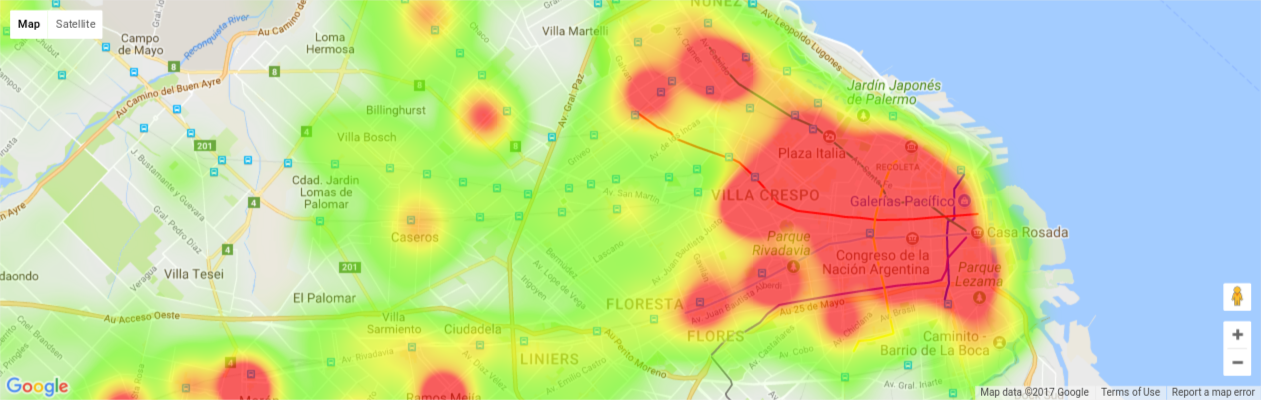
\includegraphics[width=\textwidth]{images/41}}
    				\caption{CABA con la Red de Subterráneos de Buenos Aires de fondo}
				\end{figure}
				\FloatBarrier
				
				Las zonas rojas se ubican exactamente sobre el camino de 
				los subterráneos. Sin embargo hay huecos en donde esto no ocurre. 
				Este heatmap no es suficiente como para definir un patrón aunque 
				es innegable el hecho de que la hipótesis anteriormente planteada 
				podría corresponderse. Para despejar dudas, se realiza el próximo 
				heatmap utilizando el peso de este como el precio de las propiedades 
				por metro cuadrado.			
			
				\begin{figure}
    				\centering
    				\textbf{Heatmap con el peso en el precio por metro cuadrado}\par\medskip
    				\makebox[\textwidth]{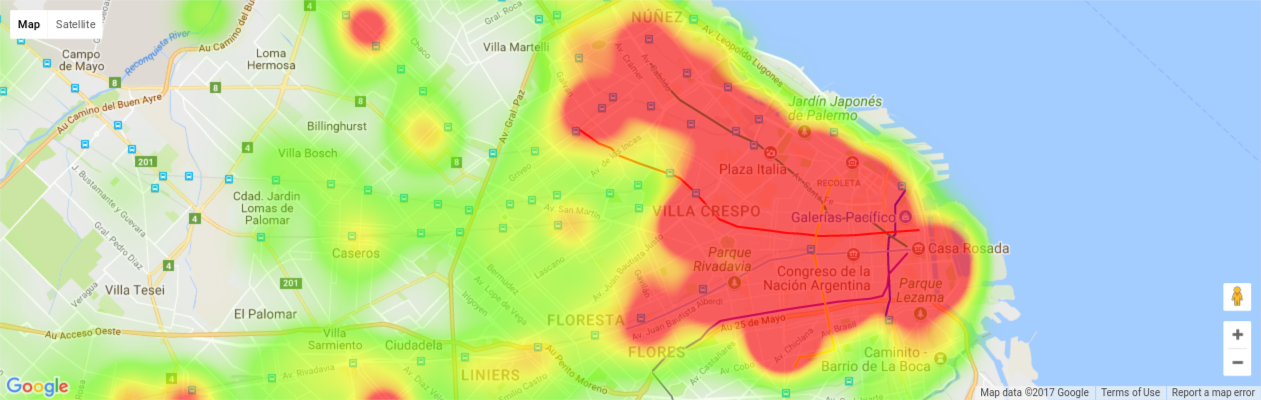
\includegraphics[width=\textwidth]{images/42}}
    				\caption{CABA con la Red de Subterráneos de Buenos Aires de fondo}
				\end{figure}
				\FloatBarrier
				
				Casi en su totalidad, las propiedades cubren las lineas de subterráneo. 
				Con la salvedad de un pequeño tramo de la linea B. Esto marca una clara tendencia en 
				la relación directa entre el precio de una propiedad con la cercanía a las 
				paradas de subterráneo en la Capital Federal.
				
		\section{Conclusiones Generales}
		
			Resumiendo, se presentan a continuación las variadas conclusiones obtenidas del análisis de 
			Google Places que serán de gran utilidad para la segunda etapa del trabajo. Se aclara que se 
			encontraron mas tendencias interesantes pero que no son de gran importancia para el 
			próximo trabajo en donde se debe aproximar el precio de una propiedad dada.			
			
			\begin{itemize}
				\item Las relaciones de precios entre CABA y GBA teniendo en cuenta todos los datos calculados 
				por Google Places siempre da una amplia mayoría en el precio de CABA contra el de GBA.
				\item Principales polos de concentración de instituciones educativas: Olivos, San Cristóbal, 
				Villa Urquiza/General Urquiza, Parque Patricios, Colegiales.
				\item En GBA se ve una tendencia a la baja de tamaños, siendo que a mayor 
				cantidad de instituciones, las propiedades tienen un tamaño menor.
				\item Las propiedades con pocos locales gastronómicos a su alrededor pertenecen a 
				GBA y prácticamente excluyen a CABA.
				\item Las propiedades con la mas grande cantidad de locales gastronómicos 
				cercanos están en su totalidad ubicados en CABA, mas particularmente su zona céntrica.
				\item Los lugares de Plaza Serrano, Recoleta, Plaza Dorrego y Belgrano 
				comparten la relación de ser centros de concentración tanto gastronómicos como culturales.
				\item En GBA las mayores concentraciones de locales gastronómicos están ubicadas 
				en la cercanía de centros comerciales (shopping centers).
				\item La cantidad de puntos de interés cultural en CABA contra los de GBA es 
				considerablemente mayor siendo 49 contra 14 las respectivas cantidades máximas.
				\item Estar alejado de los lugares "mas culturales” pero seguir perteneciendo 
				a la capital le da un valor elevado a la propiedad.
				\item En CABA hay un leve decaimiento en el precio a medida que aumenta la 
				cantidad de paradas de transporte cercanas.
				\item Existe una relación directa entre el precio de una propiedad con 
				la cercanía a las paradas de subterráneo en la Capital Federal.
\end{itemize}																	
			
\end{document}